
\section{Introduction}

The clustering problem is a basic unsupervised learning problem, and hierarchical method is probably one of the most frequently used method solving this problem. Basically, this kind of method organize the data in tree structures, and one would hope that this hierarchical structure would provide some information on the data clustering. 

Traditional hierarchical clustering algorithm \cite{hier2} is a basic bottom-up agglomerative procedure, which merges "the closest" pairs at each stage, and then iteratively organize the data into a tree structure.

However, both the traditional hierarchical algorithm and other methods ($K$-means, spectral clustering) are too restrictive. In this article, we follow an efficient modified hierarchical clustering algorithm \cite{bhc}, which involves Bayesian method. This method can be proved to have some advantages.

In this project, we begin with a basic review of traditional clustering algorithm in section 2. Then we describe the main algorithm in section 3. Theoretical supplements and of the algorithm is provided in section 4. Finally, we compare our Bayesian hierarchical method with the traditional clustering algorithm in section 5.

\section{Review of Clustering Algorithm}

\subsection{$K$-means}

The $K$-means algorithm \cite{kmeans} is one of the most classical iterative descent method which is applicable when all the variables are quantitative. Let $ D = \{ x_1, x_2, \dots, x_N \} $ be the data sets, where all the $x_i\in \re^d$ are unlabelled numeric data and $K$ is the user-specified number of clusters. The algorithm iteratively cluster the data into $K$ clusters through minimizing the following object function:
\begin{equation*}
     V=\sum_{i=1}^{K} \sum_{x_j \in C_i} d(x_j, \mu_i),
\end{equation*}
where $C_i$ is each cluster and $\mu_i$ is the arithmetic mean of the data, or the center in each cluster. To begin with, the algorithm randomly specify the center of these $K$ clusters and assign each data point to the closest cluster. Then the algorithm iteratively calculate the center after assignment, and then re-assign the data to the adjusted clusters until convergence. This cost function has several local minima and therefore several re-runs are required to obtain a cluster. 

\subsection{Spectral Clustering}

The spectral clustering algorithm \cite{spec0} and \cite{spec} is an alternative clustering method which involves the spectral method. Here, a spectral decomposition is performed to the similarity matrix whose entries are the distance or other similarity metric. Then we can choose the top few eigenvectors and project the data to the linear spans of these eigenvectors. Once the projection is done, one performs a traditional clustering ($K$-means or other methods mentioned below) to cluster these data.

\subsection{Hierarchical Clustering}

The hierarchical clustering differs greatly from the aforementioned methods of clustering. The goal here is not to find a single partitioning of the data, instead the algorithm finds the hierarchy of the data, which is usually represented as a tree. This hierarchical structure provides us with more interesting structures and we can perform partition procedures in multiple levels. 

This hierarchical algorithm has two types. The first one is agglomerative, which merges separated data at each iteration. And the other one is divisive, where the data is in one group at the beginning and are partitioned finer in each iteration. Here we introduce this traditional algorithm which organize the data in a hierarchical way. 

\begin{algorithm}
\caption{Bottom-up Hierarchical Clustering}
\KwIn{Data set $D=\{ x_1, x_2, \dots, x_N\}$ and metric $d$}
\textbf{Initialize:}  Trivial subtree $D_i=\{x_i\}$ and number of iteration $c$\;
\While(){$c>1$}{
Find the minimal distance pair of sub-trees, i.e.
\begin{equation*}
    (i_0,j_0)=\arg\min d(D_i,D_j)
\end{equation*}
Merge $D_k= D_{i_0} \cup D_{j_0}$, Delete $D_{i_0}, D_{j_0}$ and $c\leftarrow c-1$. 
}
\KwOut{A hierarchical tree structure.}
\end{algorithm}

Both these clustering algorithms possess drawbacks. The $K$-means algorithm has one fatal disadvantage that one has to specify the number of clusters, which itself is a hypothesis testing problem. For the hierarchical clustering algorithm, one fatal limitation is that we don't know at what level should we prune the tree to obtain a practical clustering. This can be improved with involving probabilistic models, which provides criterion whether the data is well organized. Moreover, probabilistic models make it possible to make predictions based on the observed data. We can use the observed data to train our model parameters via optimization and use this model to predict future data. 

\section{Bayesian Hierarchical Clustering: Algorithm}

In this section, we introduce an improved hierarchical method, which involves the Bayesian method. It's also a bottom-up agglomerative method of merging data, like the traditional hierarchical clustering. However, this modified algorithm involves Bayesian probabilistic model. Briefly speaking, this algorithm would perform a Bayesian hypothesis testing in considering a potential merge. The algorithm iteratively calculate the posterior merging probability and perform a merge on the data pair with the highest merging probability.

We now describe this algorithm in a detailed manner. Assume that the numeric data set $D=\{ x_1, x_2, \dots, x_N \}\subset \re^d$ is given. We initialize the algorithm with trivial sub-trees $\{T_i\}_{i=1}^N$, where each tree contains exactly one point $\mathcal{D}_i=\{x_i\}$. At each stage, the algorithm traverse through all the pairs of existing trees (not including the subtrees and choose one pair to perform the merge. At each merge process, the algorithm assigns new tree $T_k=(T_i,T_j)$, merging data $\mathcal{D}_k=\mathcal{D}_i \cup \mathcal{D}_j$, and delete the  $\mathcal{D}_i,\,\mathcal{D}_j$.

Here we go deeper into the selection process. For each pair of existing groups of data $D_i$ and $D_j$, we consider the potential merge $\mathcal{D}_k=\mathcal{D}_i\cup \mathcal{D}_j$ and denote $\mathcal{H}_1^k$ as the hypothesis that the all the data from group $\mathcal{D}_k$ are from one parametric distribution density $p(x|\theta)$, as opposed to generated from a mixed density $\sum \pi_i p(x|\theta_i)$. Under Bayesian scheme we place a prior $p(\theta|\beta)$ to the parameters. Therefore we can then calculate the probability of the data group $\mathcal{D}_k$ under this hypothesis as
\begin{equation*}
    p(\mathcal{D}_k|\mathcal{H}_1^k) =\int \prod_{x_i \in \mathcal{D}_k} p(x_i|\theta) p(\theta|\beta) d\theta.
\end{equation*}

The alternative hypothesis $\mathcal{H}_2^k$ is that the data in $\mathcal{D}_k$ are from different clusters. Instead of summing up over the exponentially many partitions which is often intractable, the algorithm only calculates probability of tree-consistent partitions as an approximate way. Precisely, we have
\begin{equation*}
    p(\mathcal{D}_k|\mathcal{H}_2^k)= p(\mathcal{D}_i|T_i)p(\mathcal{D}_j|T_j),
\end{equation*}
where $p(\mathcal{D}_i| T_i)$ is the probability of the dataset under a tree. We make further interpretation of this term below. If the data in $\mathcal{D}_i$ are from the same cluster, which means the hypothesis $\mathcal{H}_1^i$ is true, then it's naturally tree-consistent. Otherwise it suffices to let the left and right subtrees to be tree consistent. So we define this term recursively as follows
\begin{equation*}
    p(\mathcal{D}_k|T_k)=\pi_k p(\mathcal{D}_k|\mathcal{H}_1^k) +(1-\pi_k)p(\mathcal{D}_i|T_i)p(\mathcal{D}_j|T_j),
\end{equation*}
where $\pi_k=p(\mathcal{H}_1^k)$.

With all these in hand, we can now consider the posterior probability that $\mathcal{H}_1^k$ is true as simple application of Bayesian rule:
\begin{equation*}
    p(\mathcal{H}_k^1 |\mathcal{D}_k) = \frac{\pi_k p(\mathcal{D}_k|\mathcal{H}_1^k)}{\pi_k p(\mathcal{D}_k|\mathcal{H}_1^k)+(1-\pi_k) p(\mathcal{D}_i|T_i)p(\mathcal{D}_j|T_j)}.
\end{equation*}
We denote this quantity as $r_k=p(\mathcal{H}_k^1| \mathcal{D}_k$, and choose the largest one to perform the merge.

We present our final algorithm here, which may looks quite simple

\begin{algorithm}
    \caption{Bayesian Hierarchical Clustering}
    \KwIn{Data $\mathcal{D}=\{x_1, x_2, \dots, x_N\}$, model $p(x|\theta)$, prior $p(\theta|\beta)$}
    \textbf{Initialize:} number of clusters $c=n$, and $\mathcal{D}_i=\{x_i\}$\;
    \While{c>1}{
    For each pair $\mathcal{D}_i$ and $\mathcal{D})_j$ compute the posterior merging probability
    \begin{equation*}
        r_k=\frac{\pi_k p(\mathcal{D}_k|\mathcal{H}_1^k)}{p(\mathcal{D}_k|T_k}.
    \end{equation*}
    And find the pair $\mathcal{D}_i$ and $\mathcal{D}_j$ with maximal value.\;
    Merge $T_k\leftarrow (T_i, T_j)$ and $\mathcal{D}_k\leftarrow\mathcal{D}_i\cup \mathcal{D}_j$.
    }
    \KwOut{A Bayesian mixture model}
\end{algorithm}

\section{Theory of Bayesian Hierarchical Clustering}

We still have some problems that remain. Note that in the computation of posterior merging probability $r_k$ we actually use $\pi_k$, the prior merging probability. But we're only given the prior on the models' parameter, which is insufficient to calculate the prior merging probability. 

Here is where the Dirichlet process mixture model comes in. 

\subsection{Dirichlet Process Mixture Models}

To begin with, we briefly review the Dirichlet process mixture model, which is our generative probability model in the Bayesian hierarchical clustering model. Consider a finite mixture model with $K$ components
\begin{equation*}
    p(x|\phi)=\sum_{i=1}^K p(s=i|\mathbf{p})p(x|\theta_j).
\end{equation*}
Here $x$ is the data, $s$ is the label of this data and $\phi=(\mathbf{p}, \mathbf{\theta})$ is the model parameters. Often we would require $\theta$ to have conjugate prior, for example, if $\theta$ is the Gaussian location parameter then we would require the prior on $\theta$ to be Gaussian. The prior on the multinomial parameter $\mathbf{p}$ is the conjugate Dirichlet distribution, namely
\begin{equation*}
    p(\mathbf{p}|\alpha)=\frac{\Gamma(\alpha)}{\Gamma(\alpha/K)^K} \prod_{i=1}^K p_i^{\alpha/K -1}.
\end{equation*}
Therefore, the marginal probability of the data can be formulated as
\begin{equation*}
    p(\mathcal{D}|\alpha,\beta)=\sum_{\mathbf{s}} p(\mathbf{s}|\alpha) p(\mathcal{D}|\beta, \mathbf{s}).
\end{equation*}
Here the sum is over all possible labels. All these quantity can be well defined through a limit process, in which $K\to \infty$. Unrigorously speaking, the Dirichlet process is exactly limiting $K$ to obtain a prior, which the number of components $K$ is random and can be arbitrarily large. This extension removed the drawbacks in the $K$-means, where the number of model components should primarily specified by the user.

With this prior, we are able to compute the prior merging probability, namely $\pi_k$. Let $\mathcal{D}_k$ be the potential dataset (which is merged from other), and $n_k=|\mathcal{D}_k|$. Then the prior merging probability, which is also the prior probability for $\mathcal{H}_1^k$ is relative probability of assigning all the data in $\mathcal{D}_k$ to one components versus the probability of all other tree consistent partition. In principle we have the following
\begin{algorithm}
\caption{Algorithm for computing prior merging probability}
\textbf{Initialize:} For each leaf nodes $i$, set $d_i=\alpha$, $\pi_i=1$.\;
\ForEach{internal node k}{
compute $d_k=\alpha \Gamma(n_k)+d_{\text{left}}d_{\text{right}}$\;
$\pi_k=\alpha\Gamma(n_k)/d_k$
}
\end{algorithm}

\subsection{Properties of Approximate Inference}

We've mentioned before that our algorithm computes the posterior probability of the alternate hypothesis in an approximate way. As a matter of fact, we can prove that this approximation is valid to some extent.

We first calculate the exact inference quantity of Dirichlet process mixture model.

\begin{lemma}
    The marginal likelihood of data in the DPM is  
\begin{equation*}
    p(\mathcal{D}_k)=\sum_{v\in \mathcal{V}} \frac{\alpha^{m_v}\prod_{l=1}^{m_v} \Gamma(n_{l,v})}{\Gamma(n_k+\alpha)/\Gamma(\alpha)}\prod_{l=1}^{m_v} p(\mathcal{D}_l^v).
\end{equation*}
where $\mathcal{V}$ is the collection of all possible partitions of $\mathcal{D}_k$ and $m_v$ is the number of the clusters in partitioning $v$, $b_{l,b}$ is the number of points in cluster $l$ of partitioning $v$, abd $\mathcal{D}_l^v $ are the data points in cluster $l$ of partitioning $v$.
\end{lemma}

This lemma can be easily shown in the following manner
\begin{equation*}
    p(\mathcal{D}_k)=\sum_{v\in \mathcal{V}} p(v)p(\mathcal{D}^v),
\end{equation*}
Where $p(v)$ corresponds to the prior on the partitioning $v$ and $p(\mathcal{D}_l^v)$ corresponds to the likelihood of the partitioning under the data. Precisely, we can formulate them as follows, 
\begin{equation*}
    p(v)=\frac{\alpha^{m_v} \prod_{l=1}^{m_v} \Gamma(n_{l,v})}{\Gamma(n_k+\alpha)/\Gamma(\alpha)}.
\end{equation*}
and
\begin{equation*}
    p(\mathcal{D}^v)=\prod_{l=1}^{m_v} p(\mathcal{D}_l^v ).
\end{equation*}

Now we turn to the quantity $p(\mathcal{D}_k|T_k)$ in our approximation algorithm.

\begin{theorem}
    The quantity $p(\mathcal{D}_k|T_k)$ computed in our Bayesian Hierarchical Clustering algorithm is
    \begin{equation}
        \label{pk}
        p(\mathcal{D}_k|T_k)=\sum_{v\in \mathcal{V}_{T_k}} \frac{\alpha^{m_v}\prod_{l=1}^{m_v} \Gamma(n_{l,v})}{d_k}\prod_{l=1}^{m_v}p(\mathcal{D}_l^v),
    \end{equation}
    where $\mathcal{V}_{T_k}$ is the collection of tree-consistent partitions of $\mathcal{D}_k$ under $T_k$.
\end{theorem}

\begin{proof}
    The proof of this result is through a inductive reasoning. By the computation in Bayesian hierarchical clustering, we have
    \begin{equation*}
        p(\mathcal{D}_k|T_k)=p(\mathcal{D}_k|\mathcal{H}_1^k) \frac{\alpha \Gamma(n_k)}{d_k}+p(\mathcal{D}_i|T_i)p(\mathcal{D}_j|T_j)\frac{d_i d_j}{d_k}.
    \end{equation*}
    In this equation, the required quantity is computed recursively. So we naturally consider using an induction. First we consider the leaf nodes, which don't have subtrees, and $n_k=1, d_k=\alpha$. This implies that 
    \begin{equation*}
        p(\mathcal{D}_k|T_k)=p(\mathcal{D}_k|\mathcal{H}_1^k).
    \end{equation*}
    
    By the inductive hypothesis, we have equation \ref{pk} true for the sub-trees $T_i$ and $T_j$. And 
\end{proof}

Combining last two results to get the following 

\begin{corollary}
For any binary tree $T_k$ with the data points in $\mathcal{D}_k$ as its leaves, we have following lower bound for the marginal likelihood of a Dirichlet process mixture model:
\begin{equation*}
     \frac{d_k \Gamma(\alpha)}{\Gamma(n_k+\alpha)} p(\mathcal{D}_k|T_k )\le p(\mathcal{D}_k).
\end{equation*}
\end{corollary}

\subsection{Computational Complexity}

For now we have asserted that our approximation algorithm is practical. Moreover, the following proposition asserts that our algorithm is efficient.

\begin{proposition}
    The number of the tree-consistent partitions is exponential in the number of the data points for the balanced binary tree.
\end{proposition}

\begin{proof}
    Assume that our balanced binary tree is of depth $l$, then the number of the data is of $\mathcal{O}(2^l)$. On the other hand, assume that $T_i$ has $C_i$ tree-consistent partitions of $\mathcal{D}_i$ and $T_j$ has $C_j$, then the number of the tree-consistent partitions for $T_k=(T_i,T_j)$ of data $\mathcal{D}_k$ is $C_i C_j+1$. For each leaf nodes $C_i=1$, these implies that the tree-consistent partitions of the whole tree grows in $\mathcal{O}(2^{2^l})\approx \mathcal{O}(2^n)$.
\end{proof}
 
\section{Application to Real Data}

In this section we use the aforementioned clustering method to study a real world data. Here the data we use is \href{https://www.kaggle.com/rohan0301/unsupervised-learning-on-country-data}{country socio-economic data} from Kaggle. This dataset stores the social-economic index and health factors of each country. Our object is to categorize these countries for the NGO to make practical aids. 

The whole dataset contains 167 countries and 9 features and we list them as follows
\begin{itemize}
    \item child\_mort: Death of children under 5 years of age per 1000 live births.
    \item exports: Exports of goods and services per capita. Given as \%age of the GDP per capita.
    \item health: Total health spending per capita. Given as \%age of GDP per capita.
    \item imports: Imports of goods and services per capita. Given as \%age of the GDP per capita.
    \item income: Net income per person.
    \item inflation: The measurement of the annual growth rate of the Total GDP.
    \item life\_expec: The average number of years a new born child would live if the current mortality patterns are to remain the same.
    \item total\_fer: The number of children that would be born to each woman if the current age-fertility rates remain the same.
    \item gdpp: The GDP per capita. Calculated as the Total GDP divided by the total population.
\end{itemize}

This clustering problem doesn't have a real version of labels, and the number of the clusters are unspecified. We begin with the traditional hierarchical clustering.

\begin{figure}[H]
    \caption{Traditional Hierarchical Clustering Result}
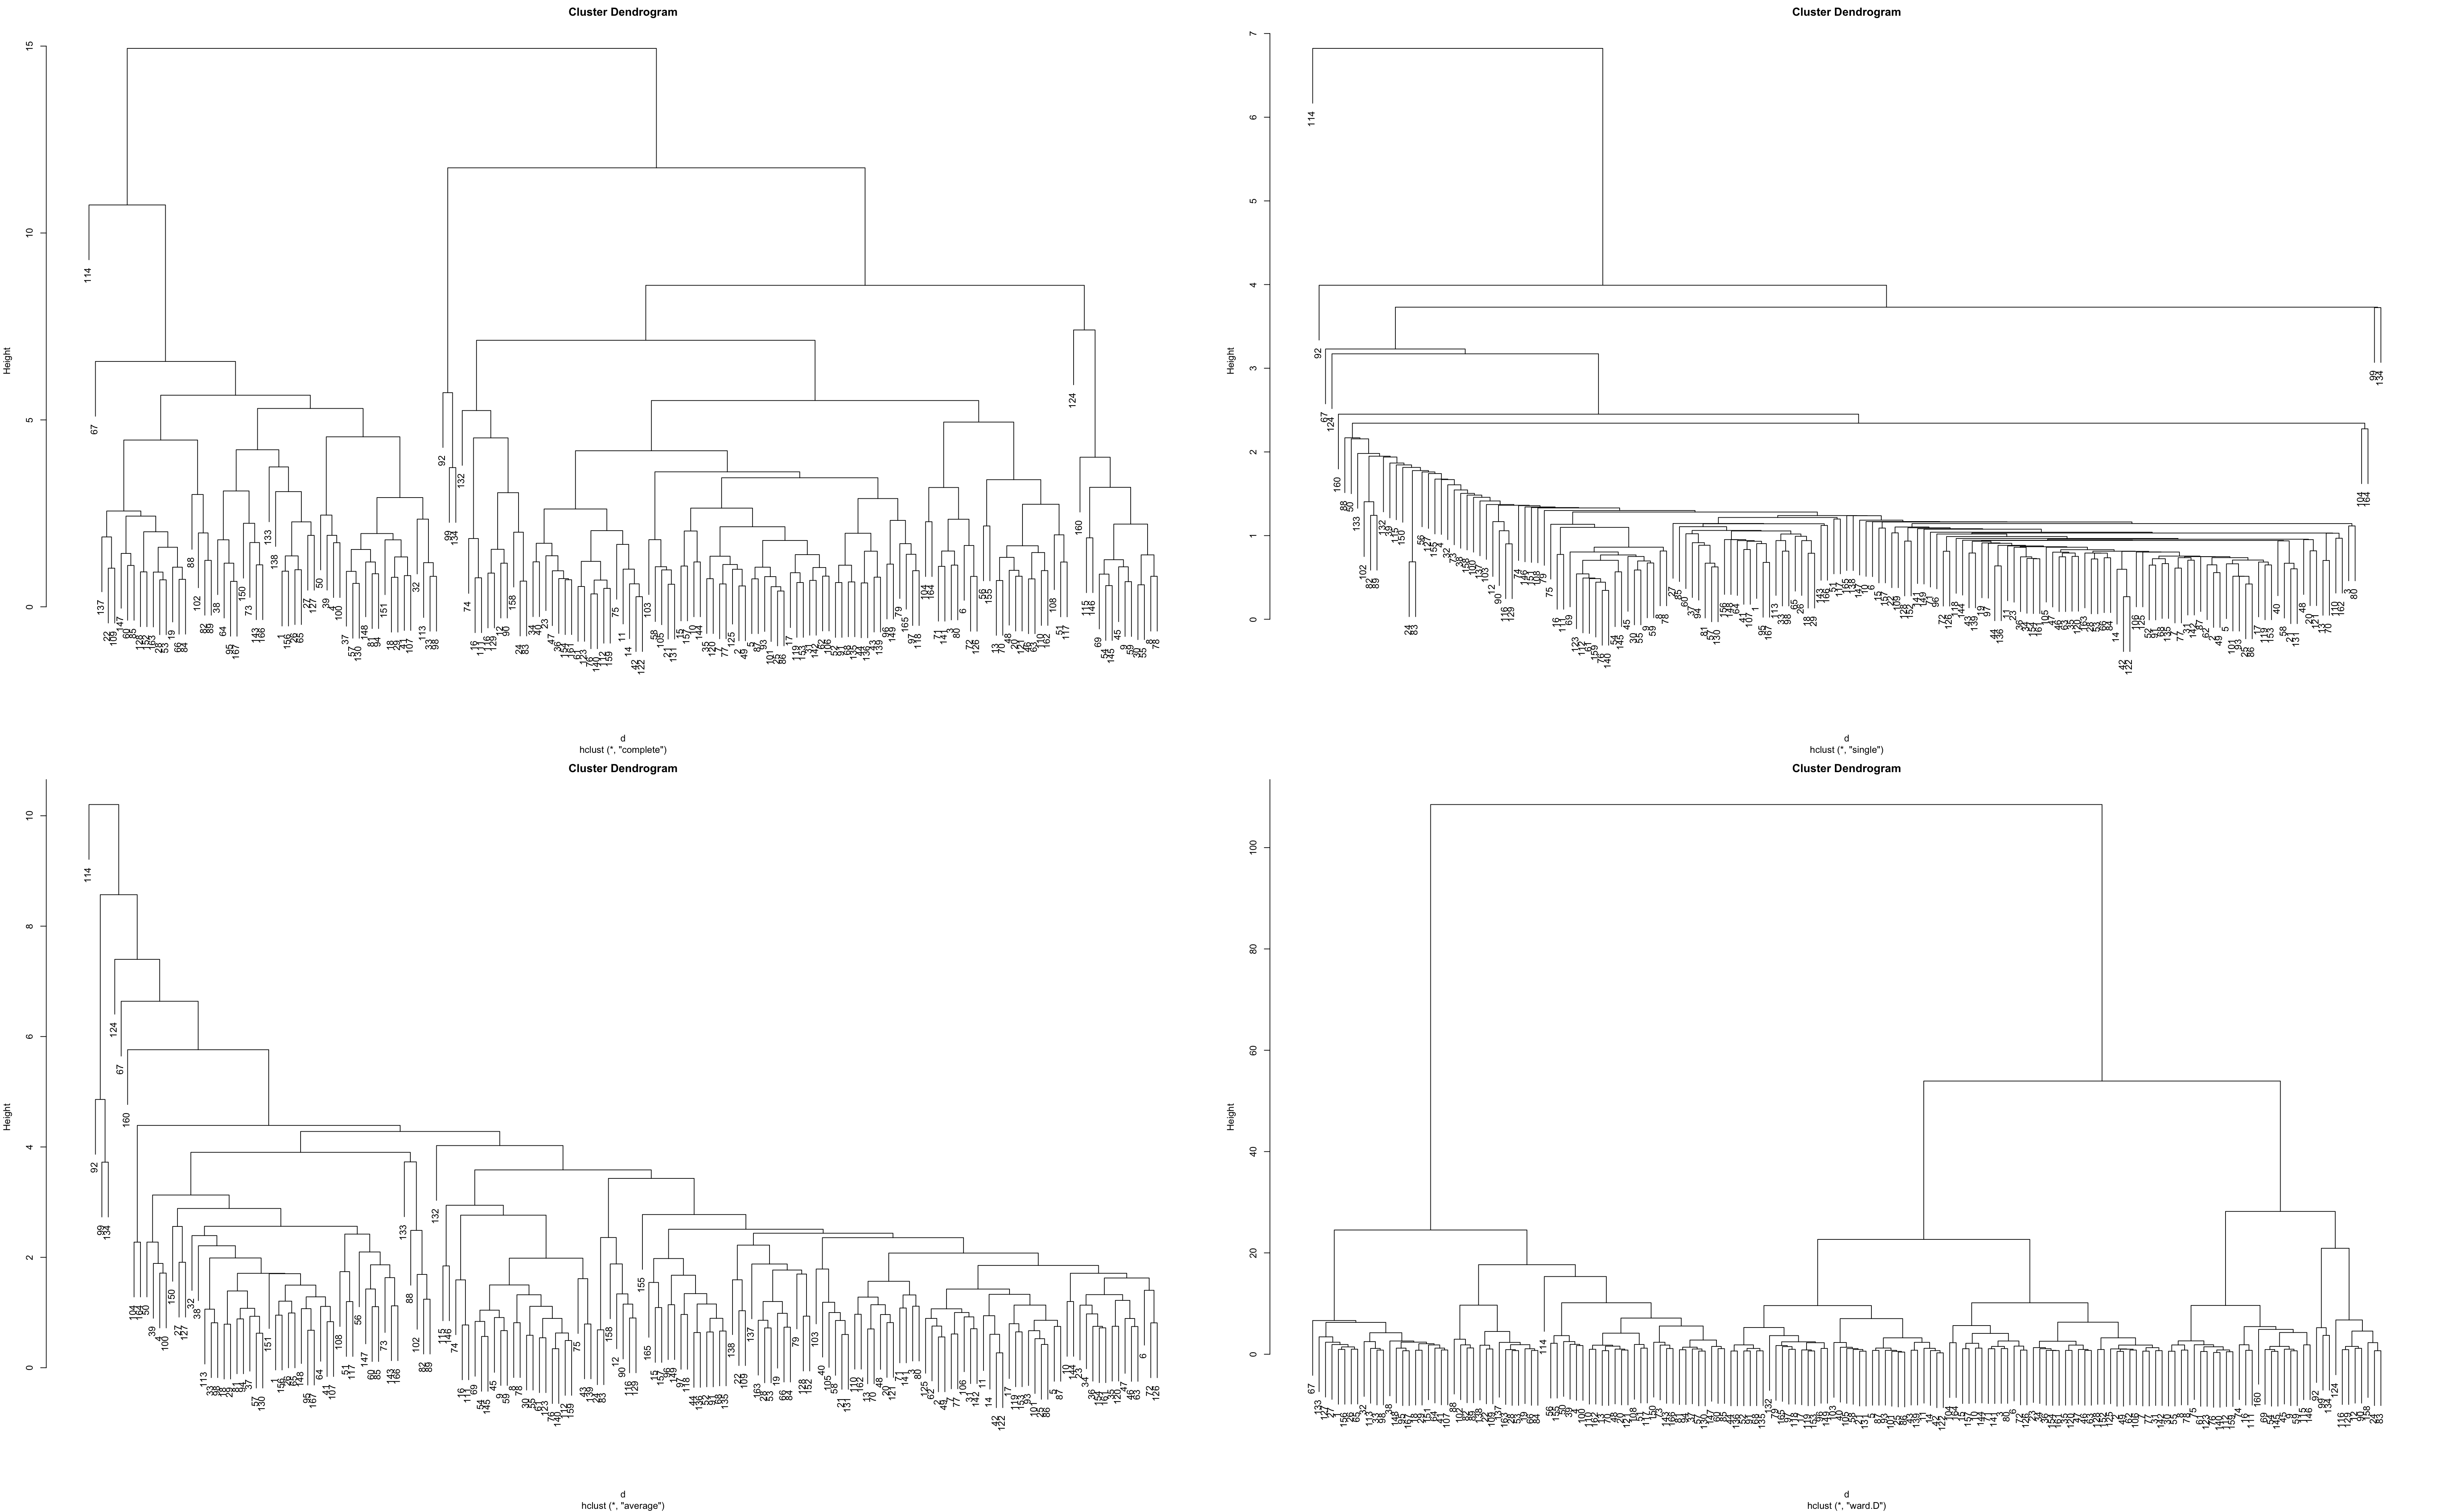
\includegraphics[width=\textwidth]{00003f.png}
\caption*{These four figures are the dendrogram output of the tradition hierarchical clustering algorithm, with different metric function.}
\end{figure}
These dendrogram implies that the structures of these trees are very disordered. Different metric would actually result in very different tree structures. And this disordered tree structure makes the clusters unidentifiable. Indeed, different levels of cut would also cause the clustering results to be different, this leads to the intractability. Intuitively, the Ward's method gives the best, or at least most organized dendrogram. The agglomerative coefficients are listed below.
\begin{table}[H]
    \caption{Agglomerative Coefficients}
    \begin{tabular}{l|cccc}
                                                  & Single Linkage & Average Linkage & Complete Linkage & Ward's Distance \\\hline
    AC & 0.843          & 0.875           & 0.913            & 0.952          
    \end{tabular}
    \end{table}
Now let's consider the Bayesian hierarchical clustering to be used in this data. From the dendrogram plotted above and below, we see that the BHC algorithm creates a more organized tree structure. This advantage is more significant in the higher level.
\newpage

\begin{figure}[H]
    \caption{Bayesian Hierarchical Clustering Result}
    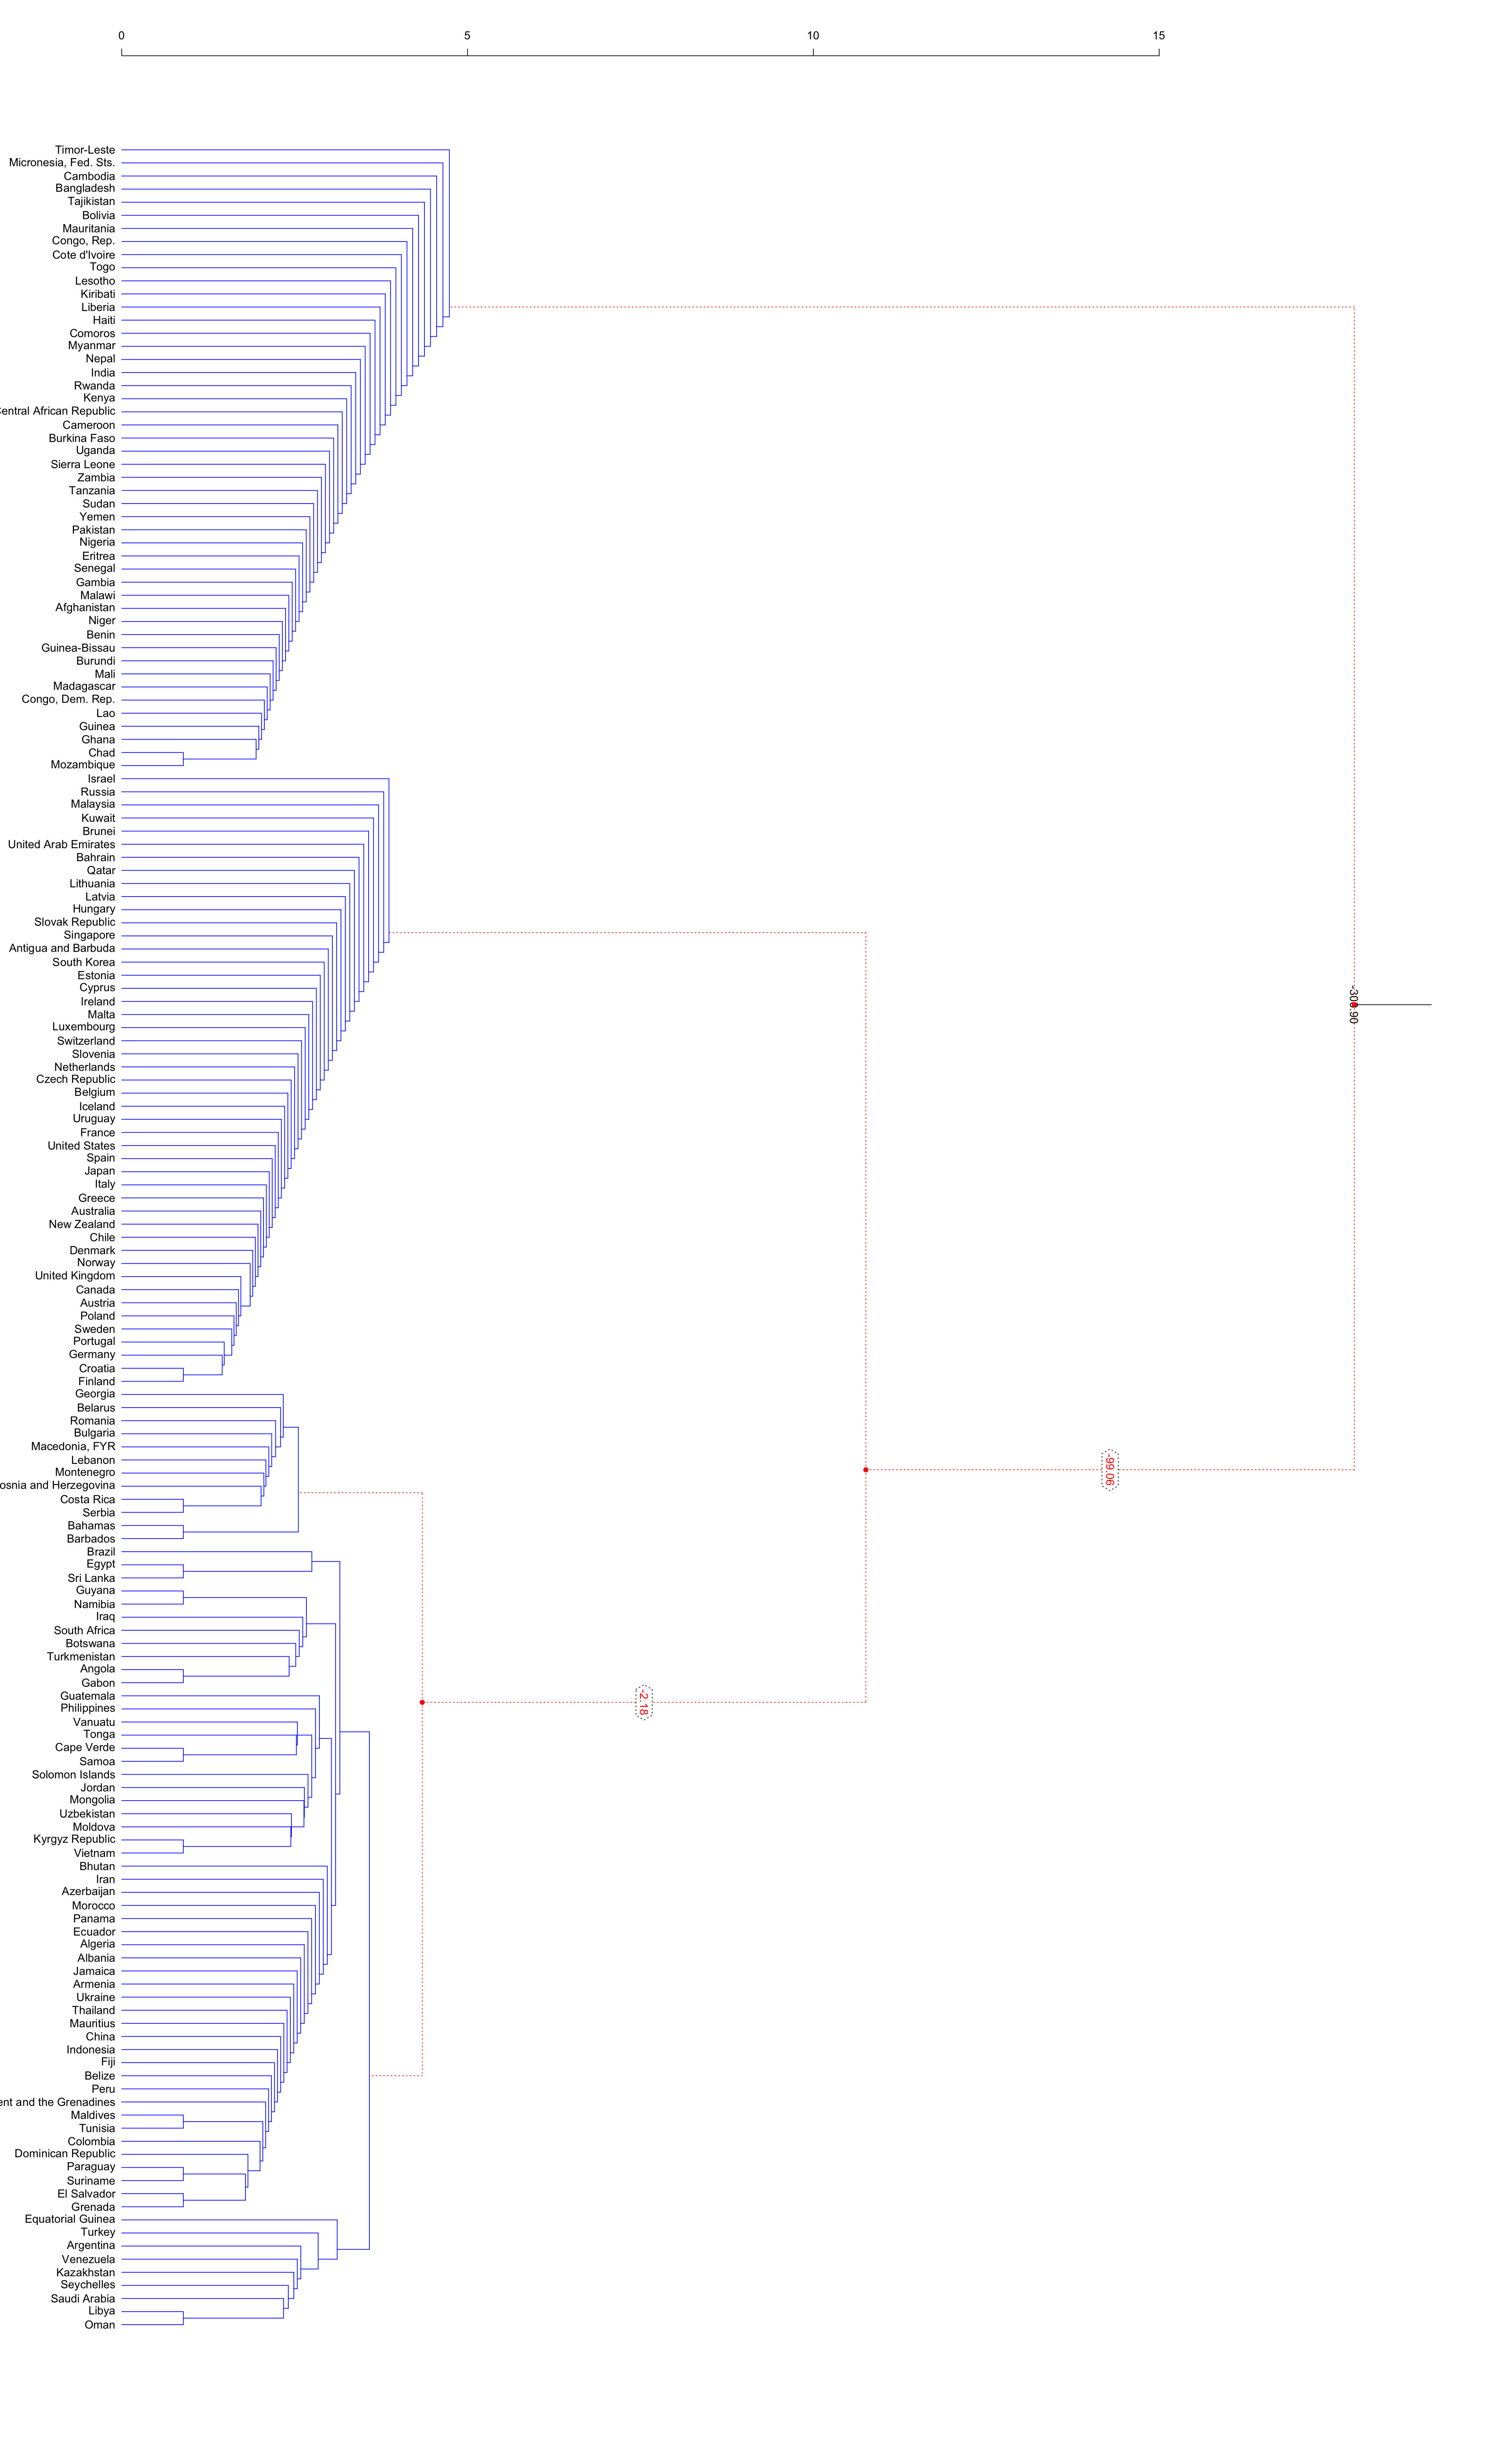
\includegraphics[width=\textwidth]{000005.png}
\end{figure}


